\documentclass[10pt,handout,xcolor=pdftex,dvipsnames,table]{beamer}
%\usepackage{pgfpages}
%\mode<handout>{\setbeamercolor{background canvas}{bg=black!0}}
%\pgfpagesuselayout{2 on 1}[A4paper,border shrink=1mm]

\mode<presentation> {
\setbeamertemplate{background canvas}[vertical shading][bottom=blue!10,top=white!10]
%%%%%%%%%%%%%%%%%%%%%%%%%%%%%%%%%%%%%%%%%%
\usetheme[secheader]{Boadilla}
%\usetheme{Szeged}
  \setbeamercovered{transparent}

%\usetheme{Frankfurt}
%\usetheme{Singapore}
%\usetheme{CambridgeUS}
\usecolortheme[RGB={7,81,145}]{structure}
}
\usepackage[english]{babel}
% or whatever
%\usepackage[latin1]{inputenc}
% or whatever
\usepackage{ colortbl}
\usepackage{times}
\usepackage[T1]{fontenc}
\usepackage[applemac]{inputenc}
%\usepackage{hyperref}
 \usepackage[usenames,dvipsnames]{pstricks}
 \usepackage{epsfig}
 \usepackage{pst-grad} % For gradients
 \usepackage{pst-plot} % For axes
\usepackage{eurosym}
\setbeamercovered{transparent}
\usepackage{amsmath}
\usepackage{hyperref}
\usepackage{tikz}
%%%%
\usepackage[usenames,dvipsnames]{pstricks}
\usepackage{epsfig}
\usepackage{pst-grad} % For gradients
\usepackage{pst-plot} % For axes
\usepackage{graphicx}





%\usebackgroundtemplate{\includegraphics[width=\paperwidth,height=\paperheight]{./stein.jpg}
%%%%
% Or whatever. Note that the encoding and the font should match. If T1
% does not look nice, try deleting the line with the fontenc.
%\title[The impact of firms' subsidies] % (optional, use only with long paper 

\title[Dose-response analysis] % (optional, use only with long paper titles)
{ 
Are you spending enough? A dose-response analysis of regional R\&D subsidies}
\subtitle{
}

\author[Gabriele R.] % (optional, use only with lots of authors)
{Marco Corsino$^1$, %^1 %\inst{},
{\bf Roberto Gabriele$^2$}, %^2, %\inst{Department of Management, University of Bologna} and 
Anna Giunta$^3$
Giovanni Cerulli$^4$%^3 %\inst{Department of Economics, University Roma 3}
}

% - Give the names in the same order as the appear in the paper.
% - Use the \inst{?} command only if the authors have different
%   affiliation.

\institute[AY 2024/2025] % (optional, but mostly needed)
{$^1$ Department of Management, University of Milano Bicocca

$^2$ Department of  Economics and Management, University  of  Trento


$^3$ Department of Economics, University Roma Tre
$^4$ IRCrES CNR, Roma

%\vspace{1cm}

}
% - Use the \inst command only if there are several affiliations.
% - Keep it simple, no one is interested in your street address.
\date[3/2/2025] % (optional, should be abbreviation of conference name)
{\footnotesize Methods and Applications for Empirical Economics Academic Year 2024/2025, 

Ph.D. Programme in Economics and Finance, UniTn \& UniBZ}
% - Either use conference name or its abbreviation.
% - Not really informative to the audience, more for people (including
%   yourself) who are reading the slides online

% This is only inserted into the PDF information catalog. Can be left
% out. 
% If you have a file called "university-logo-filename.xxx", where xxx
% is a graphic format that can be processed by latex or pdflatex,
% resp., then you can add a logo as follows:
 \pgfdeclareimage[height=0.6cm]{university-logo}{./Figs/newlogo_unitn_it.png}
 \subject{Dose-response analysis}
 \logo{\pgfuseimage{university-logo}}
% Delete this, if you do not want the table of contents to pop up at
% the beginning of each subsection:
\AtBeginSubsection[]
{
  \begin{frame}<beamer>
    \frametitle{Outline of the talk}
    \tableofcontents[currentsection,currentsubsection]
  \end{frame}
}
\begin{document}
{
% \usebackgroundtemplate{ \tikz\node[opacity=0.2]  {
\includegraphics[width=\paperwidth]{./Figs/Logo_Universita_di_Trento.jpg}};}
\begin{frame}
%\vspace{1.8cm}  
\titlepage


\end{frame}
}
%%%%%%%%%%%%%%%%%%%%%%%%
\begin{frame}
  \frametitle{Outline}
  \tableofcontents
  % You might wish to add the option [pausesections]
\end{frame}
%%%%%%%%%%%%%%%%%%%%%%%%%%%%%%%%%%%%%%%%%%%%%%%%%%%
\section{Introduction}
%%%%%%%%%%%%%%%%%%%%%%%%%%%%%%%%%%%%%%%
\begin{frame}
\frametitle{A preamble: The reasons for market failures}
\framesubtitle{And their solution}
\begin{block} {The innovation process of firm is costly, uncertain and not fully appropriable:}
	\begin{itemize}
		\item Firm private innovation investments can never be fully appropriated  (other firms have the opportunity to free ride)
	\end{itemize}
\end{block}
	This leads to:
	\begin{itemize}
 		\item  Underinvestment in individual R\&D activities
	\end{itemize}
\begin{block} {At aggregate level:} 
	The R\&D expenditure will be below the socially desirable level
\end{block}
\begin{block} {Public intervention aims at:} 
	\begin{itemize}
		\item Let some socially  desirable R\&D projects valuable for private investors to a level at which it becomes profitable for companies to invest
	\end{itemize}
\end{block}
\end{frame}
%%%%%%%%%%%%%%%%%%%%%%%%%%%%%%%%%%%%%%%%%%
%%%%%%%%%%%%%%%%%%%%%%%%%%%%%%%%%%%%%%%
\begin{frame}
\framesubtitle{The economic rationale behind the subsidies to Innovation activity}
\frametitle{Introduction}
	\begin{block}{Common justification for government intervention to engender innovation (Lundvall and Borras, 2005):}
		\begin{itemize}
		\item Enhance economic activity and stimulate growth, 
		\item Upgrade the quality of human resources, and 
		\item Promote firm competitiveness (especially wrt local contexts) 
		%\item What is still contended, however, is the ability of policy makers to rectify market failures, provide effective incentives to spur welfare-enhancing innovations, and avoid the introduction of additional distortions in the economic system
		\end{itemize}
	\end{block}	
	
	\begin{block}{What is still contended, however, is the ability of policy makers}
		\begin{itemize}
			\item To provide effective incentives to spur welfare-enhancing innovations, and 
			\item Avoid the introduction of additional distortions in the competitive arena 		\item To rectify {\bf market failures}, 
		\end{itemize}
	\end{block}	
\end{frame}
%%%%%%%%%%%%%%%%%%%%%%%%%%%%%%%%%%%%%%%%%%%
%%%%%%%%%%%%%%%%%%%%%%%%%%%%%%%%%%%%%%%%%%%%%%
\begin{frame}{Empirical evidence}
{Additionality of R\&D subsidies}
Results on additionality for R\&D programs in Italy: 
\begin{enumerate}
\item Caloffi, Mariani and Sterlacchini (2016):
"[...] Several types of programmes yield non-negligible probability of success and that the outcome variable used to measure programme impact matters. 

If there exist any differential in probability of success between the government levels that may deliver the programmes, {\bf this differential is favourable to  regional governments}"
\end{enumerate}
\begin{block}{The last observation  is the starting point of the present analysis!}
\end{block}	
\end{frame}
%%%%%%%%%%%%%%%%%%%%%%%%%%%%%%%%%%%%%%%%%%%%%%
%%%%%%%%%%%%%%%%%%%%%%%%%%%%%%%%%%%%%%%%%%%%%%
\begin{frame}{Empirical evidence II}
{Additionality of R\&D subsidies across countries}
There exists a rich stream of literature summarized by Meta Analysis: 
\begin{enumerate}
\item Garcia-Quevedo, J. (2004) 
\item Negassi and Sattin (2014)
\item Castellacci and Mee Lie (2015)
\item Gaillard-Ladinska et al. (2015)
\end{enumerate}
{\bf Recent studies:} 
Aristei, D., Sterlacchini, A., Venturini, F. (2016) provide evidence about European countries: no crowding out, but no additionality


In general: Mixed results 

(read: there conditions that enable additionality to be taken into account...)

\end{frame}
%%%%%%%%%%%%%%%%%%%%%%%%%%%%%%%%%%%%%%%%%%%%%%
%%%%%%%%%%%%%%%%%%%%%%%%%%%%%%%%%%%%%%%%%%%%%%
\begin{frame}{What about R\&D subsidies intensity?}
{Empirical evidence using Dose-Response}
Few studies: 
\begin{enumerate}
\item Marino, M., Lhuillery, S., Parrotta, P., Sala, D. (2016): 
{\it either no additionality or substitution effects between public and private R\&D expenditure. Crowding-out effects appear to be more pronounced for medium-high levels of public subsidies}
\item Dai and Cheng (2015): {\it there exists a saturation point beyond which a further increase in public subsidies does not yield an increase of firm's total R\&D investment. Moreover, a minimum threshold value of public subsidies is required to induce the firm's private R\&D spending}
\end{enumerate}

{\it obs: data requirements are a binding constraint}

\begin{block}{ We would contribute to this stream of literature}
To provide to the policy maker finer results and more precise indications
\end{block}

\end{frame}
%%%%%%%%%%%%%%%%%%%%%%%%%%%%%%%%%%%%%%%%%%%%%%
%%%%%%%%%%%%%%%%%%%%%%%%%%%%%%%%%%%%%%%
\begin{frame}
\frametitle{Research question(s) and objective of the study}
\begin{block} {Context: }Trentino (Italy) Provincial Law 6/99
\end{block}
\begin{block} {Scope and time window of evaluation:}  R\&D subsidies granted to firms from year 2002 to 2007
\end{block}
%\begin{block} {Research question:} 
%	\begin{itemize}
%		\item Is there evidence of additionality in innovative effort?
%	\end{itemize}
%\end{block}

\begin{block} {Research questions:}
\begin{enumerate}
\item Do different intensities of subsidies imply different effects on additionality? 

%{\footnotesize In particular, does the program of R\&D   subsidies in Trentino during the years 2002-2008 lead to additionality of innovative efforts?}
\item What kind of R\&D investments present evidence of additionality and for "which doses of the treatment"?
\end{enumerate}
\end{block}


\end{frame}
%%%%%%%%%%%%%%%%%%%%%%%%%%%%%%%%%%%%%%%%%%

%%%%%%%%%%%%%%%%%%%%%%%%%%%%%%%%%%%%%%%%%%%
\begin{frame}
\frametitle{The advantages of our study}
\begin{block} {Exhaustive information about subsidies:}
		 Detailed informations about all the direct financial incentives granted to Trentino firms
\end{block}

\begin{block} {No confounding effects: }
	\begin{itemize}
		\item No overlapping among the different levels of industrial policy
		\item We exactly know  if and when each firm was  subsidized and the timing of their expenses
\end{itemize}
\end{block}

%\begin{block} {Unique data availability:}  Possibility to merge different database to conduct the evaluation exercises
% \end{block}
\end{frame}
%%%%%%%%%%%%%%%%%%%%%%%%%%%%%%%%%%%%%%%%
%%%%%%%%
%%%%%%%%%%%%%%%%%%%%%%%%%%%%%%%%%%%%%%%%%%%
\begin{frame}
\frametitle{The context of study: The PL 6/99 in Trentino}
\framesubtitle{Some key details}
{\footnotesize
\begin{block} {The procedure to get financed:}
\begin{itemize}
	\item Submit a Research project to APIAE
\item A technical committee decides whether the project can be financed or not

{\it If yes:}
\item A financial committee decides whether the financial and economic requests are adequate for the project
\end{itemize}
\end{block}
\begin{block} { Timing of expenses:}
'' $\left[...\right]$ Le spese relative alle domande esaminate con procedura valutativa devono essere effettuate dal giorno successivo la domanda di agevolazione ed entro tre anni dalla data di concessione dell'agevolazione''
\end{block}
%\begin{block} { Additionality in the PL 6/99:}
%'' $\left[...\right]$sia finalizzato ad attivit\`a di ricerca supplementari, che si aggiungano a quelle da essa normalmente svolte nel quadro delle proprie attività correnti''
%\end{block}
}
\end{frame}
%%%%%%%%%%%%%%%%%%%%%%%%%%%%%%%%%%%%%%%%%%%%%
%%%%%%%%%%%%%%%%%%%%%%%%%%%%%%%%%%%%%%%%%%%%%%
\begin{frame}{The distribution of grants intensity}
{Years 2002-2007}
\begin{figure}[t]
\centering
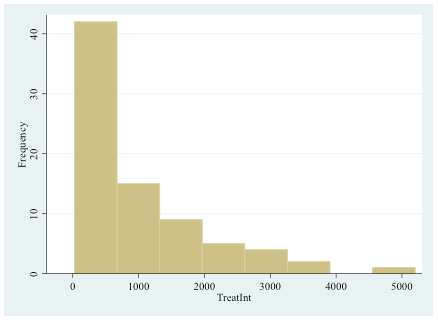
\includegraphics[width=.8\textwidth]{./Figs/TIdistr.png}
\end{figure}
\end{frame}
%%%%%%%%%%%%%%%%%%%%%%%%%%%%%%%%%%%%%%%%%%%%%%
\section{Data}
%%%%%%%%%%%%%%%%%%%%%%%%%%%%%%%%
\begin{frame}
\frametitle{Data}
\framesubtitle{The collection of information for the evaluation exercise}

\begin{block} {The database:} 
\begin{itemize}

\item It is the results from the merge of three archives:
		\begin{itemize}
		\item Administrative data from APIAE
		\item AIDA data (BvD) + Pitagora + Telemaco (for integrations)$^1$
		\item ASIA data (ISTAT)
		\end{itemize}
\item It covers the years 2001-2008 and 
\end{itemize}
\end{block}

%\begin{block} {Unique data availability:}  Possibility to collect exhaustive data to conduct the evaluation exercises on different aspects related with the issues 
%\end{block}

{\footnotesize $^1$: We solved many problems of different formats and conventions.}
\end{frame}
%%%%%%%%%%%%%%%%%%%%%%%%%%%%%%%%%%%%%%%%%%%%
\begin{frame}{Variables}
we consider the following outcome variables to study additionality:
\begin{enumerate}
\item Employment dynamics (Empl) - the number of employees;
\item  Total labor costs (TC);
\item  Unit labor costs (ULC) - the ratio between net labor costs and the total number of employees; 
\item  Capital expenses (FA) - the net tangible assets expenses;
\item  Intangible intensity (IA) - the net intangible assets expenses.
\end{enumerate}
what does it mean ''net''...
\end{frame}
%%%%%%%%%%%%%%%%%%%%%%%%%%%%%%%%%%%%%%%%%%%%%%
%%%%%%%%%%%%%%%%%%%%%%%%%%%%%%%%%%%%%%%%%%%%%%
\begin{frame}{Controls}
 The exogenous confounders included in our models are all lagged one year and comprise:
\begin{itemize}
\item unit labor costs;
\item 	size of firm as measured by the number of employees;
\item	rescaled cashflow as a proxy of the financial constraints that firms face, measured as the ratio between cash flow and total sales;
\item capital intensity 
\item a control variable (year) for controlling business cycle effects;
\end{itemize}

\end{frame}
%%%%%%%%%%%%%%%%%%%%%%%%%%%%%%%%%%%%%%%%%%%%%%
%%%%%%%%%%%%%%%%%%%%%%%%%%%%%%%%%%%%%%%%%%%%%%
\begin{frame}{A regression approach}
We start from a specific population generating process for the two exclusive potential outcome



$w=1: y_1=\mu_1+g_1({\bf x})+h(t)+e_1$ 

$w=0: y_0=\mu_0+g_0({\bf x})+e_0$

It can be shown using the Rubin framework that: 

$y_i= \mu_0+w_i ATE+x_i\delta_0+w_i (x_i -{\bf x})\delta+w_i (h(_{ti})-\bar{h})\eta_i  $
\end{frame}
%%%%%%%%%%%%%%%%%%%%%%%%%%%%%%%%%%%%%%%%%%%%%%
%%%%%%%%%%%%%%%%%%%%%%%%%%%%%%%%%%%%%%%%%%%%%%
\begin{frame}{Estimation}
Starting from the previous linear relationship we aim at estimating:

$ E(y_i | w_i,h_{ti},x_i)=\mu_0+w_i ATE+x_i\delta_0+w_i(x_i-\bar{x} )\delta+w_i(h(t_i)-\bar{h})  $ (a)

\begin{itemize}
\item Ordinary Least Squares (OLS) can be used to get consistent estimation of all parameters of interest in (a)
\item  h(t) is specified as follow:

$h(t)=a t+ b t^2 + ct^3$

\end{itemize}



\end{frame}
%%%%%%%%%%%%%%%%%%%%%%%%%%%%%%%%%%%%%%%%%%%%%%
%%%%%%%%%%%%%%%%%%%%%%%%%%%%%%%%%%%%%%%%%%%%%%%%%%%%
%%%%%%%%%%%%%%%%%%%%%%%%%%%%%%%%%%%%%%%%%%%%%%
\begin{frame}{The model implementation}
\begin{figure}[t]
\centering
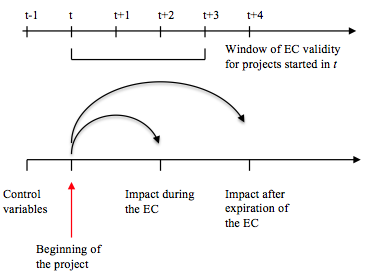
\includegraphics[width=0.75\textwidth]{./Figs/SchemaMod.png}
\end{figure}
\end{frame}

%%%%%%%%%%%%%%%%%%%%%%%%%%%%%%%%%%%%%%%%%%%%%
%%%%%%%%%%%%%%%%%%%%%%%%%%%%%%%%%%%%%%%%%%%%%%
\begin{frame}{The model implementation II}
\begin{enumerate}
\item What is the "dose"?
\item (example a firm that receives 1,500\euro as a subsidy for a project that costs 2000\euro,  75\% of percentage of subsidization)
\item Options:
\item S level:  S=1500
\item Total expenses of project: P=2000
\item P percentage Pp=75
\end{enumerate}
We have chosen S level

nonetheless to be clear:

1500 is 75\% of 2000, but also 10\% of 15000 for instance!

{\bf Different measures give different answers!}
\end{frame}

%%%%%%%%%%%%%%%%%%%%%%%%%%%%%%%%%%%%%%%%%%%%%

\section{Results}
%%%%%%%%%%%%%%%%%%%%%%%%%%%%%%%%%%%%%%%%%%%%%%
\begin{frame}{Impact on labour}
Impact on employment level
\begin{figure}[t]
\centering
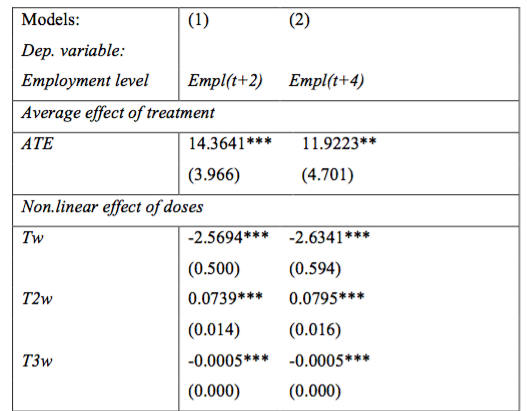
\includegraphics[width=0.7\textwidth]{./Figs/T1.png}
\end{figure}
\end{frame}
%%%%%%%%%%%%%%%%%%%%%%%%%%%%%%%%%%%%%%%%%%%%%%
%%%%%%%%%%%%%%%%%%%%%%%%%%%%%%%%%%%%%%%%%%%%%%
\begin{frame}{Impact on labour}
Impact on employment level
\begin{figure}[t]
\centering
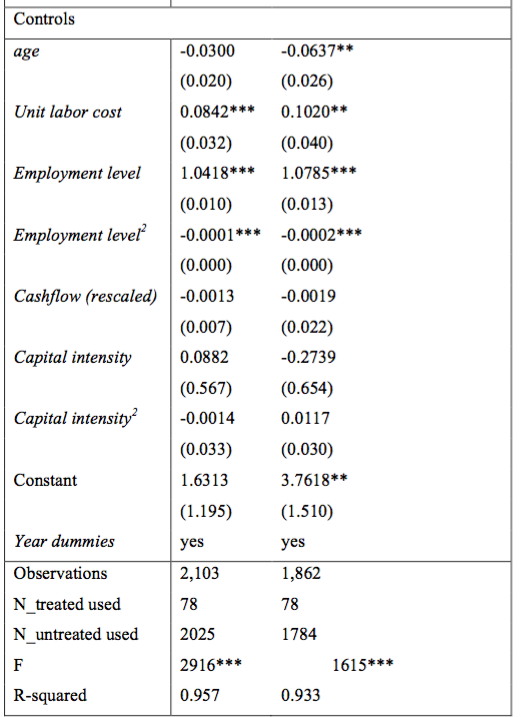
\includegraphics[width=0.5\textwidth]{./Figs/T2.png}
\end{figure}
\end{frame}
%%%%%%%%%%%%%%%%%%%%%%%%%%%%%%%%%%%%%%%%%%%%%%
%%%%%%%%%%%%%%%%%%%%%%%%%%%%%%%%%%%%%%%%%%%%%%
\begin{frame}{Impact on labour}
Impact on employment level
\begin{figure}[t]
\centering
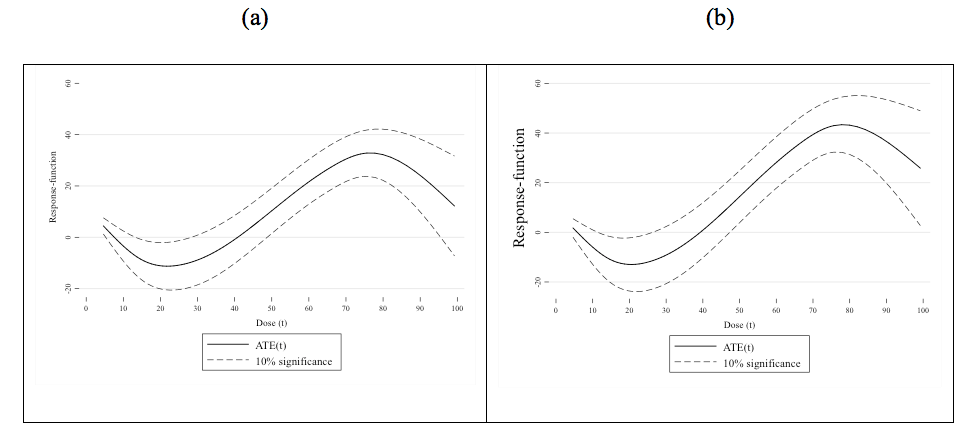
\includegraphics[width=1\textwidth]{./Figs/EL1.png}
\end{figure}
\end{frame}
%%%%%%%%%%%%%%%%%%%%%%%%%%%%%%%%%%%%%%%%%%%%%%
%%%%%%%%%%%%%%%%%%%%%%%%%%%%%%%%%%%%%%%%%%%%%%
\begin{frame}{Impact on labour}
Impact on employment level
\begin{figure}[t]
\centering
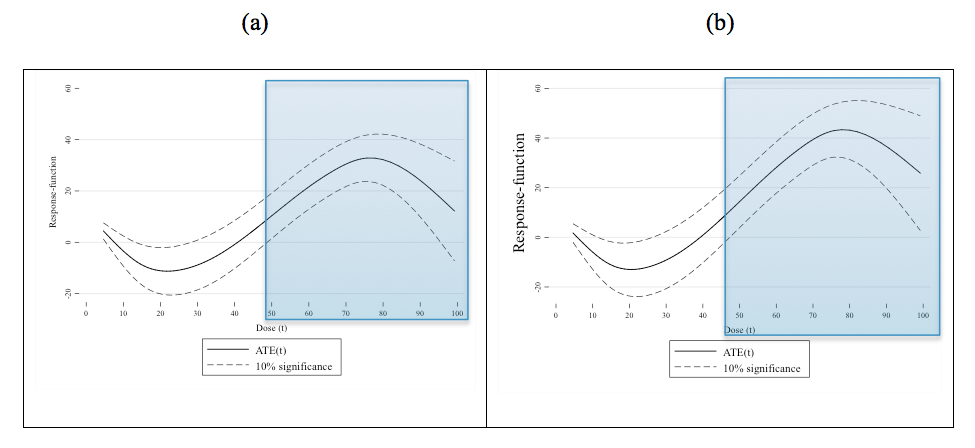
\includegraphics[width=1\textwidth]{./Figs/EL1shad.png}
\end{figure}
\end{frame}
%%%%%%%%%%%%%%%%%%%%%%%%%%%%%%%%%%%%%%%%%%%%%%
%%%%%%%%%%%%%%%%%%%%%%%%%%%%%%%%%%%%%%%%%%%%%%
\begin{frame}{Impact on labour}
Impact on wage costs
\begin{figure}[t]
\centering
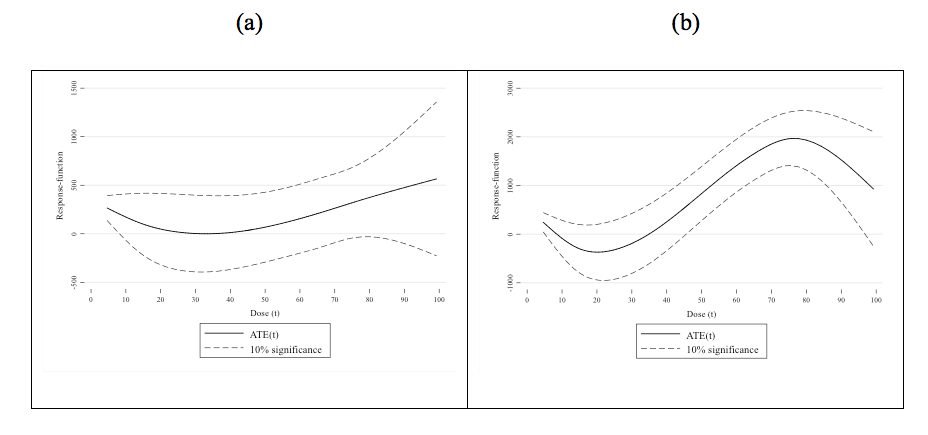
\includegraphics[width=1\textwidth]{./Figs/TLC.png}
\end{figure}
\end{frame}
%%%%%%%%%%%%%%%%%%%%%%%%%%%%%%%%%%%%%%%%%%%%%%
%%%%%%%%%%%%%%%%%%%%%%%%%%%%%%%%%%%%%%%%%%%%%%
\begin{frame}{Impact on labour}
Impact on wage costs
\begin{figure}[t]
\centering
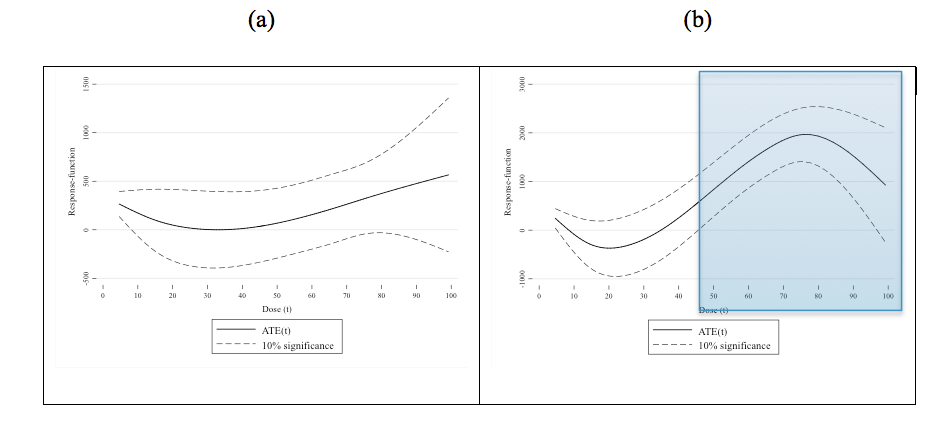
\includegraphics[width=1\textwidth]{./Figs/TLCshad.png}
\end{figure}
\end{frame}
%%%%%%%%%%%%%%%%%%%%%%%%%%%%%%%%%%%%%%%%%%%%%%%%%%%%%%%%%%%%%%%%%%%%%%%%%%%%%%%%%%%%%%%%%%%%



\begin{frame}{Impact on labour}
Impact on unit labor costs
\begin{figure}[t]
\centering
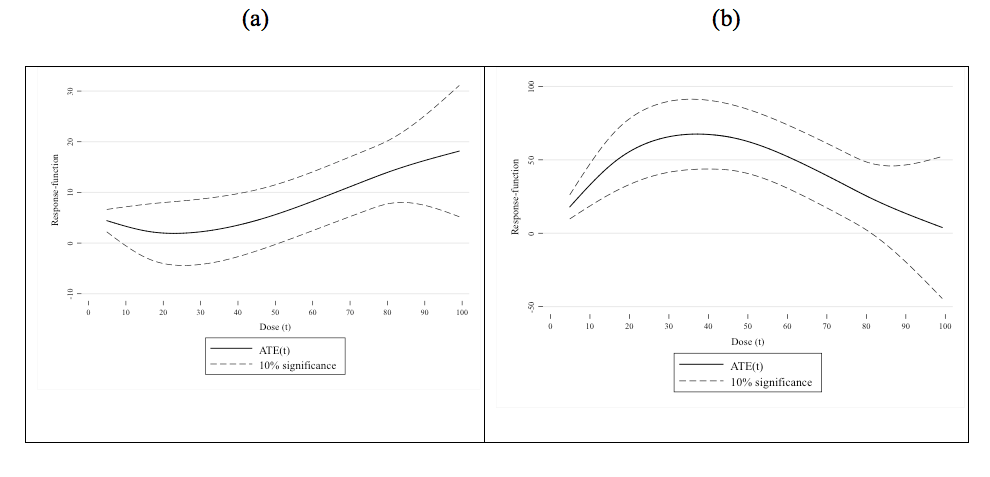
\includegraphics[width=1\textwidth]{./Figs/ULC.png}
\end{figure}
\end{frame}
%%%%%%%%%%%%%%%%%%%%%%%%%%%%%%%%%%%%%%%%%%%%%%
%%%%%%%%%%%%%%%%%%%%%%%%%%%%%%%%%%%%%%%%%%%%%%%
\begin{frame}{Impact on labour}
Impact on unit labor costs
\begin{figure}[t]
\centering
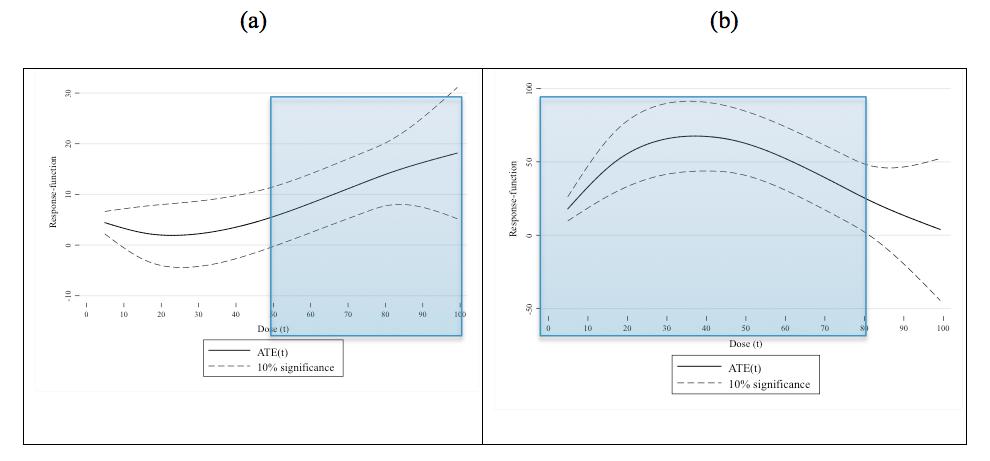
\includegraphics[width=1\textwidth]{./Figs/ULCshad.png}
\end{figure}
\end{frame}
%%%%%%%%%%%%%%%%%%%%%%%%%%%%%%%%%%%%%%%%%%%%%%
%%%%%%%%%%%%%%%%%%%%%%%%%%%%%%%%%%%%%%%%%%%%%%
\begin{frame}{Impact on capitalized expenses}
Impact on fixed assets investment
\begin{figure}[t]
\centering
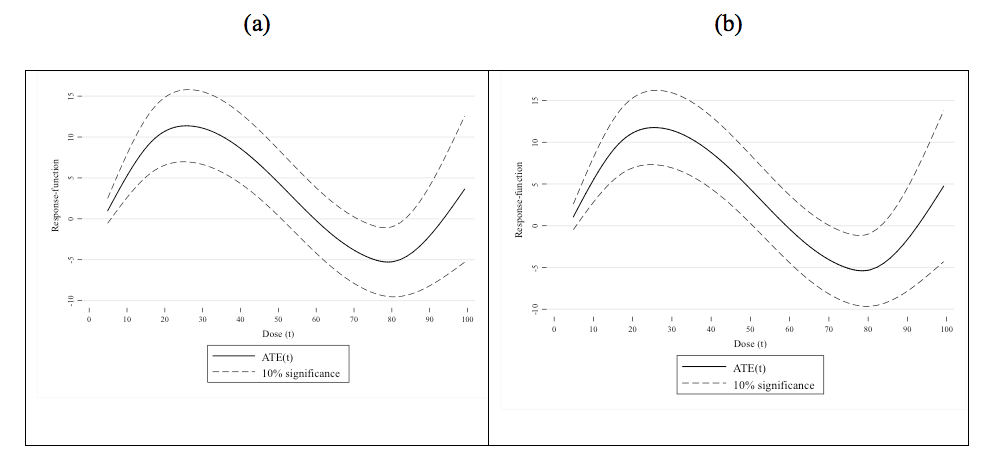
\includegraphics[width=1\textwidth]{./Figs/FA.png}
\end{figure}
\end{frame}
%%%%%%%%%%%%%%%%%%%%%%%%%%%%%%%%%%%%%%%%%%%%%%
%%%%%%%%%%%%%%%%%%%%%%%%%%%%%%%%%%%%%%%%%%%%%%
\begin{frame}{Impact on capitalized expenses}
Impact on fixed assets investment
\begin{figure}[t]
\centering
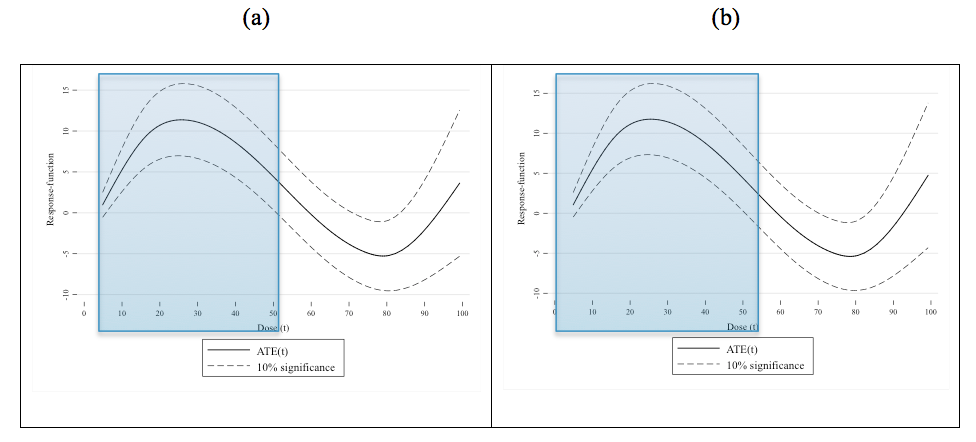
\includegraphics[width=1\textwidth]{./Figs/FAshad.png}
\end{figure}
\end{frame}
%%%%%%%%%%%%%%%%%%%%%%%%%%%%%%%%%%%%%%%%%%%%%%
%%%%%%%%%%%%%%%%%%%%%%%%%%%%%%%%%%%%%%%%%%%%%%
\begin{frame}{Impact on capitalized expenses}
Impact on intangible assets investment
\begin{figure}[t]
\centering
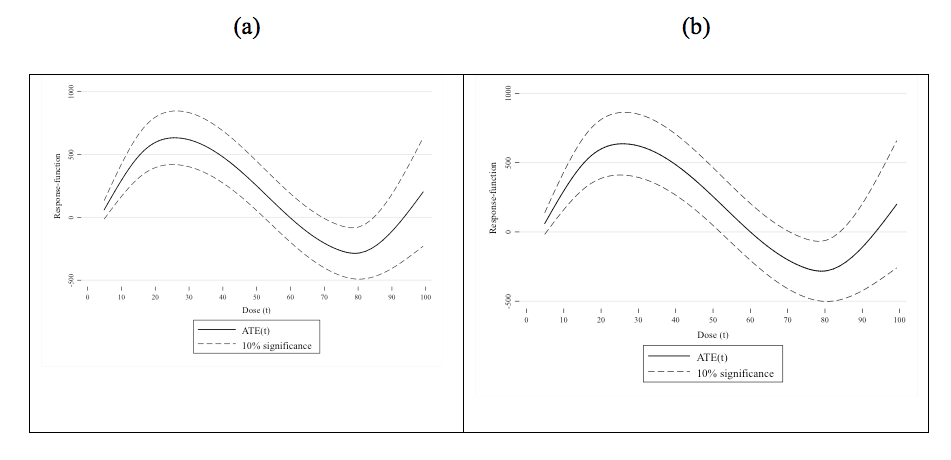
\includegraphics[width=1\textwidth]{./Figs/IA.png}
\end{figure}
\end{frame}
%%%%%%%%%%%%%%%%%%%%%%%%%%%%%%%%%%%%%%%%%%%%%%%%%%%%%%%%%%%%%%%%%%%%%%%%%%%%%%%%%%%%%%%%%%%
\begin{frame}{Impact on capitalized expenses}
Impact on intangible assets investment
\begin{figure}[t]
\centering
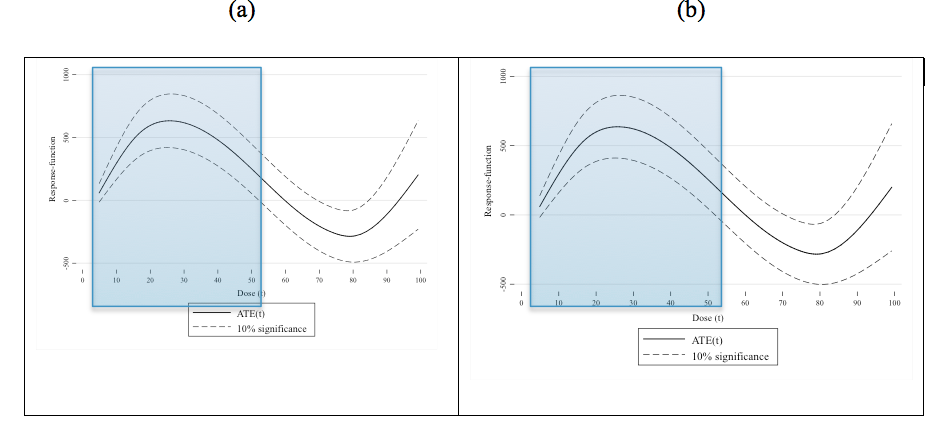
\includegraphics[width=1.0\textwidth]{./Figs/IAshad.png}
\end{figure}
\end{frame}
%%%%%%%%%%%%%%%%%%%%%%%%%%%%%%%%%%%%%%%%%%%%%%

%
%%%%%%%%%%%%%%%%%%%%%%%%%%%%%%%%%%%%%%%%
\section{Discussion and Future Perspectives}
\begin{frame}
\frametitle{Discussion of results}
\begin{block}{Major results} There is evidence of additionality of innovative efforts:
\begin{itemize}
\item on fixed assets and intangibles intensity
\item on employment levels and on composition of human resources (higher skill employed)
\end{itemize}

\end{block}
Moreover: 

\begin{block}{}
\begin{itemize}
\item higher doses are associated with employment related effects
\item smaller doses are associated with capitalized investments
\end{itemize}

\end{block}
\end{frame}
%%%%%%%%%%%%%%%%%%%%%%%%%%%%%%%%%%%%%%%%
%\begin{frame}
%\frametitle{Conclusions}
%\begin{block}{There is evidence of additionality:}
%On intangible assets (one and two years after the treatment)
%\end{block}
%
%
%\begin{block}{Performance:}
%\begin{itemize}
%\item  No effects on performances as measured by:
%Size, labor costs,
%Impact on 
% profitability
%
%\item Positive effect after three years on Labor productivity (total sales per employee)
%\end{itemize}
%\end{block}
%The accounting standards can be responsible for the dification of the profitability index
%\end{frame}
%%%%%%%%%%%%%%%%%%%%%%%%%%%%%%%%%%%%%%%%
%\section{Discussion and Future Perspectives}
\begin{frame}
\frametitle{Future research agenda}
\begin{block}{Results extensions:}
\begin{itemize}
\item Use longer time series to see the effect of crisis
\item Take into consideration longer lags to evaluate the impact on performances 
\item merge data about R\&D workers (difficult to obtain)
\end{itemize}
\end{block}
from methodological point of view:

deepen the robustness checks of results
\end{frame}

\begin{frame}
	\frametitle{Thanks for your attention}

%\begin{block}{Comments and suggestions are welcome!}

%\end{block}



\begin{block}{For further information:}

\begin{itemize}
			\item roberto.gabriele@unitn.it 
\end{itemize}

\end{block}
\end{frame}


\end{document}


